\documentclass[10pt, a4paper]{article}
\usepackage[utf8]{inputenc}
\usepackage[T1]{fontenc,url}
\usepackage{multicol}
\usepackage{multirow}
\usepackage{parskip}
\usepackage{lmodern}
\usepackage{microtype}
\usepackage{verbatim}
\usepackage{amsmath, amssymb}
\usepackage{tikz}
\usepackage{physics}
\usepackage{mathtools}
\usepackage{algorithm}
\usepackage{algpseudocode}
\usepackage{listings}
\usepackage{enumerate}
\usepackage{graphicx}
\usepackage{float}
\usepackage{hyperref}
\usepackage{tabularx}
\usepackage{siunitx}
\usepackage{fancyvrb}
%\usepackage{natbib}
%\bibliographystyle{dinat}
\usepackage[makeroom]{cancel}
\usepackage[margin=2.0cm]{geometry}
\usepackage{pdfpages}
\usepackage[margin=10pt, textfont={small, it}, labelfont={bf}, labelsep=endash]{caption}
\renewcommand{\baselinestretch}{1}



\begin{document}
\title{COMAP - Compression of level 1 files}
\author{
    \begin{tabular}{r l}
        Jonas Gahr Sturtzel Lunde & (\texttt{jonassl})
    \end{tabular}}
% \date{}    % if commented out, the date is set to the current date

\maketitle
% Code found at \url{https://github.com/asdfbat/AST5220/tree/master/Project}
% \vspace{0.7cm}
\begin{figure}[H]
    \centering
    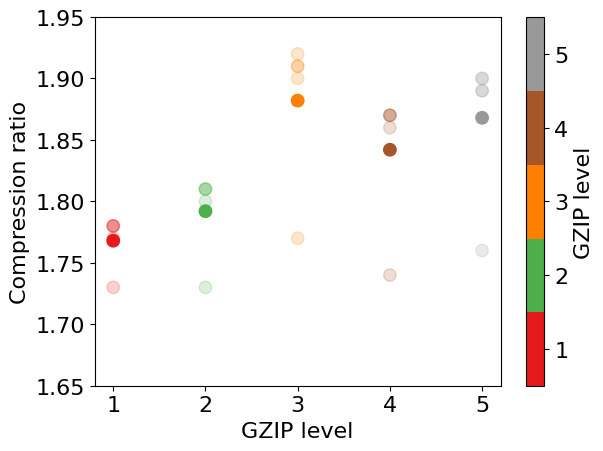
\includegraphics[scale=0.55]{gzip_compratio.png}
    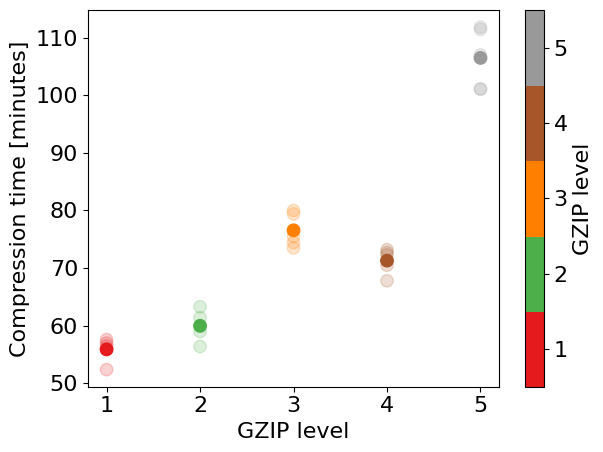
\includegraphics[scale=0.55]{gzip_comptime.png}
    \caption{}
    \label{}
\end{figure}

\begin{figure}[H]
    \centering
    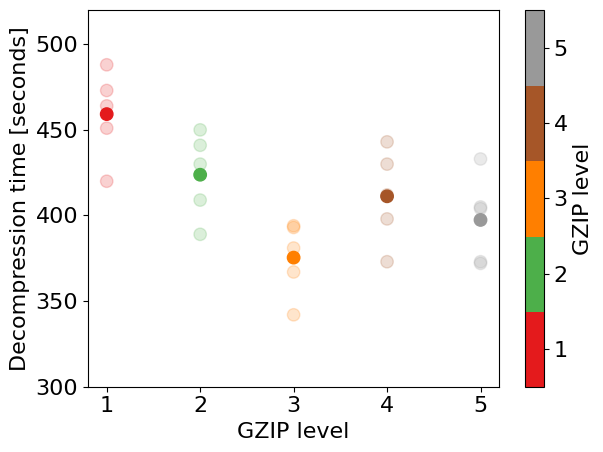
\includegraphics[scale=0.55]{gzip_decomptime.png}
    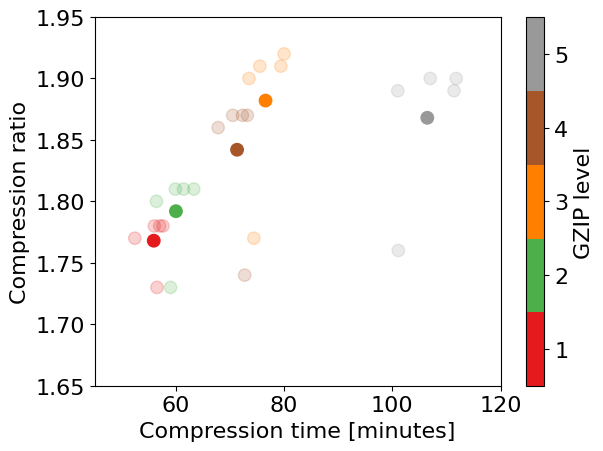
\includegraphics[scale=0.55]{comptime_compratio.png}
    \caption{}
    \label{}
\end{figure}


\end{document}